\documentclass[10pt,a4paper]{article}
\usepackage[margin=0.95in]{geometry}
\usepackage[T1]{fontenc}
\usepackage{lmodern}
\usepackage{microtype}
\usepackage{amsmath,amssymb,amsthm,mathtools}
\usepackage{booktabs,enumitem,float,graphicx}
\usepackage{xcolor,tikz}
\usetikzlibrary{arrows.meta,positioning,calc}
\usepackage[hidelinks]{hyperref}

\definecolor{bluefill}{RGB}{231,240,250}
\definecolor{greenfill}{RGB}{234,246,237}
\definecolor{redline}{RGB}{166,48,48}
\newtheorem{theorem}{Theorem}
\newtheorem{lemma}[theorem]{Lemma}
\newtheorem{proposition}[theorem]{Proposition}
\newtheorem{corollary}[theorem]{Corollary}
\newtheorem{remark}[theorem]{Remark}
\newcommand{\U}{\mathcal U}
\newcommand{\F}{\mathcal F}
\newcommand{\Oset}{\mathcal O}
\newcommand{\Sset}{\mathcal S}
\newcommand{\Top}{\operatorname{Top}}
\newcommand{\cost}{\operatorname{cost}}
\newcommand{\col}{\operatorname{col}}

\title{COMPASS: Prefix Realization under Routing Preferences\\
\large A step-by-step account of the conflict graph and its bounds}
\author{Loqman Salamatian}
\date{November 2026}

\begin{document}
\maketitle

\begin{abstract}
COMPASS selects ingress infrastructure and steers traffic using a limited number of BGP prefixes. Unlike direct traffic assignment, a prefix exposes the same set of announcing ingresses to every user group using it; each group then chooses its preferred ingress. We formalize the deployment and routing decisions, then study a two-stage approach: first compute a desirable assignment assuming direct control, and then determine how many prefixes are needed to reproduce it. A conflict graph captures exactly which intended assignments cannot share a prefix, making the minimum number of prefixes its chromatic number. We show that even second-choice assignments can require arbitrarily many prefixes, although never more than logarithmically many in the number of ingresses used, and identify two kinds of preference agreement that restore constant bounds. Finally, we address the case where the available prefix budget is too small to preserve every assignment.
\end{abstract}

\section{A prefix is a shared menu}

Suppose COMPASS would like to send user group $U$ through ingress $B$, although $U$ ranks the options $A\succ_U B\succ_U C$. If only $B$ announces the prefix given to $U$, then the resulting route is $B$. If both $A$ and $B$ announce it, the resulting route is $A$. COMPASS chooses the \emph{set of visible options} and then users select which of these options they pick (hence the menu analogy!).

This distinction matters when prefixes are shared. Putting two user groups on the same prefix makes both groups see the union of the ingresses needed by their intended assignments. An ingress desired by one group may be preferred over the intended ingress of the other. In that case, the two assignments cannot both be preserved by that prefix.

There are therefore two separate questions:
\begin{enumerate}[leftmargin=*,itemsep=2pt]
\item \textbf{Infrastructure selection:} which facilities and ingress options should carry the traffic if COMPASS could assign demand directly?
\item \textbf{Prefix realization:} with those options selected, which user assignments can share a BGP prefix without changing the resulting routes?
\end{enumerate}
We first state the joint model to make its assumptions explicit. Figure~\ref{fig:flow-to-conflict} then explains how its selected flow becomes the assignment grid used to construct a conflict graph. The main combinatorial results concern this graph for a fixed deployment and target assignment.

\section{Optimization model and decomposition}
\label{sec:model}

\subsection{Inputs and decisions}

Let $\U$ denote user groups, with traffic weights $w_U>0$. Let $\mathcal P$ be the set of peers (neighboring networks) and $\F$ the set of candidate facilities, with elements $f\in\F$. The possible ingress options are peer--facility pairs $\Oset\subseteq\mathcal P\times\F$: an option is $o=(P,f)$ for a peer $P\in\mathcal P$, and $f(o)$ denotes its facility. Throughout, ``option'' and ``ingress'' are synonyms for $o\in\Oset$. Sending one unit of traffic from $U$ through $o$ incurs penalty $\phi(o,U)$. Option $o$ and facility $f$ have capacities $\kappa_o$ and $\kappa_f$. Opening facility $f$ costs $c_f$, and serving traffic incurs per-unit operating costs $b_o$ and $b_f$. At most $B_{\rm prefix}$ prefix identifiers can be used.

The joint model has three kinds of decisions:
\begin{center}
\small
\begin{tabular}{@{}llp{0.57\linewidth}@{}}
\toprule
\textbf{Decision} & \textbf{Variables} & \textbf{Meaning}\\
\midrule
Deployment & $x_f,y_o\in\{0,1\}$ & Open facility $f$; activate option $o$.\\
Announcements & $z_{o,k}\in\{0,1\}$ & Option $o$ announces prefix $k$.\\
Assignment & $\lambda_{U,k},r_{U,o,k}\in[0,1]$ & Fraction of $U$ assigned prefix $k$; fraction of $U$ served by $o$ through $k$.\\
\bottomrule
\end{tabular}
\end{center}
Write $a_o(U)=\sum_{k=1}^{B_{\rm prefix}} r_{U,o,k}$ for the total fraction of group $U$ served by option $o$. A fractional $\lambda_{U,k}$ splits one group across several prefixes. BGP gives each network a single best route per prefix, so such a split assumes the group can be steered at a finer grain, for example by handing different destination prefixes to parts of the group through DNS. If each group must use a single prefix, take $\lambda_{U,k}\in\{0,1\}$. We assume every group has a \emph{strict, prefix-independent} preference ranking. The notation $o'\succ_U o$ means that $U$ prefers $o'$ to $o$; equivalently, $\pi_o(U)$ denotes a numerical preference score that increases with desirability. This assumption is essential to the graph-coloring analysis below; if rankings depend on the prefix, the graph must be defined differently. The model is the routing model of the main COMPASS paper in the special case where every group can reach every announcing ingress and rankings do not depend on the prefix; there, Lemma~\ref{lem:color} below is that paper's exact-realization lemma.

\subsection{Joint formulation}

A natural objective is to minimize total routing penalty:
\begin{equation}\label{eq:objective}
\min\ \sum_{U\in\U}\sum_{o\in\Oset}w_U\phi(o,U)a_o(U).
\end{equation}
Its constraints are
\begin{align}
\sum_{k=1}^{B_{\rm prefix}}\lambda_{U,k}&=1 &&\forall U,\label{eq:group}\\
\sum_{o\in\Oset}r_{U,o,k}&=\lambda_{U,k} &&\forall U,k,\label{eq:balance}\\
r_{U,o,k}&\le z_{o,k}\le y_o\le x_{f(o)} &&\forall U,o,k,\label{eq:enable}\\
r_{U,o,k}&\le 1-z_{o',k} &&\forall U,k,o,o'\text{ with }o'\succ_U o,\label{eq:dominance}\\
a_o(U)&=\sum_{k=1}^{B_{\rm prefix}} r_{U,o,k} &&\forall U,o,\label{eq:aggregate}\\
\sum_U w_Ua_o(U)&\le\kappa_o y_o &&\forall o,\label{eq:ocap}\\
\sum_{o:f(o)=f}\sum_U w_Ua_o(U)&\le\kappa_fx_f &&\forall f.\label{eq:fcap}
\end{align}
Equations~\eqref{eq:group}--\eqref{eq:balance} allocate all demand. Equation~\eqref{eq:enable} permits traffic only on announcing, active, deployed options. Equation~\eqref{eq:dominance} is the crucial BGP-choice constraint: traffic from $U$ cannot use $o$ on prefix $k$ if an option $o'$ preferred by $U$ also announces $k$. Equations~\eqref{eq:ocap}--\eqref{eq:fcap} limit the loads induced by those winners.

The monetary deployment and operating cost is
\begin{equation}\label{eq:money}
C(x,y,a)=\sum_{f}c_fx_f
+\sum_f b_f\sum_{o:f(o)=f}\sum_Uw_Ua_o(U)
+\sum_o b_o\sum_Uw_Ua_o(U),
\end{equation}
which may be constrained by a deployment budget $C(x,y,a)\le C_{\max}$. We assume every user can use every prefix identifier; otherwise, a prefix-availability constraint must also be imposed.

The problem contains two distinct combinatorial optimization problems. Even without BGP routing preferences, selecting capacitated facilities and assigning demand is NP-hard once deployment is limited by the budget $C_{\max}$ or charged opening costs $c_f$ in the objective; with neither, opening every facility is optimal. Even for a fixed deployment and target assignment, determining the minimum number of prefixes required to realize that assignment exactly is equivalent to graph coloring, which is also NP-hard.

The second difficulty arises because prefix announcements couple routing decisions across users: adding an option to a prefix can redirect traffic from other options, potentially increasing routing cost or violating capacity constraints.

\subsection{A two-stage approach}
\label{sec:two-stage}

\paragraph{Stage 1: select infrastructure under full control.}
Ignore the prefix limit and allow COMPASS to send arbitrary fractions $a_o(U)$ of each user group directly to active options. For any \emph{fixed} deployment, this is a minimum-cost flow on
\[
s\longrightarrow\U\longrightarrow\Oset_{\rm active}
\longrightarrow\F_{\rm open}\longrightarrow t.
\]
The source supplies $w_U$ at each user, a $U\to o$ arc has unit cost $\phi(o,U)$, an $o\to f(o)$ arc has capacity $\kappa_o$, and an $f\to t$ arc has capacity $\kappa_f$. The per-unit operating costs $b_o$ and $b_f$ can be added to the corresponding arcs when they belong to the objective. When they appear only in the budget $C(x,y,a)\le C_{\max}$, moving that constraint into the objective with a Lagrange multiplier gives the same flow problem for each multiplier value; the opening costs $c_f$ are fixed once the deployment is fixed. A feasible flow sending $\sum_U w_U$ units is the optimal divisible assignment for that \emph{fixed} deployment. Selecting the deployment itself remains a discrete search.

Let $D\subseteq\Oset$ be the selected options and let $a^\star_o(U)$ be the resulting full-control target.

\paragraph{Stage 2: realize the target using prefixes.}
For each positive fraction $a^\star_o(U)$, introduce an \emph{atomic intended assignment} $v=(U,o)$ with traffic weight $w_v=w_Ua^\star_o(U)$. The word ``atomic'' refers only to the realization step: we treat this component as one item to be assigned to one prefix. If several components share a prefix, all their intended options announce that prefix. Each component is then routed to its most preferred announcing option. We ask how to partition these components into no more than $B_{\rm prefix}$ prefixes while preserving their intended routes, or minimizing the loss when exact preservation is impossible.

Figure~\ref{fig:flow-to-conflict} follows one toy assignment through these representations. In the full-control flow network, the three selected user-to-ingress arcs carry $U_1\to B$, $U_2\to C$, and $U_3\to A$. The middle panel records these positive flows as filled cells in a user-by-ingress grid. It also marks each user's first choice, which is not the target in this example. The right-hand panel keeps only the selected assignments and joins two whenever sharing a prefix would cause one group to choose the other's ingress instead.
% --- Figure 1: flow -> ranked assignment matrix -> conflict graph ---
\begin{figure}[tbp]
\centering
\resizebox{\linewidth}{!}{%
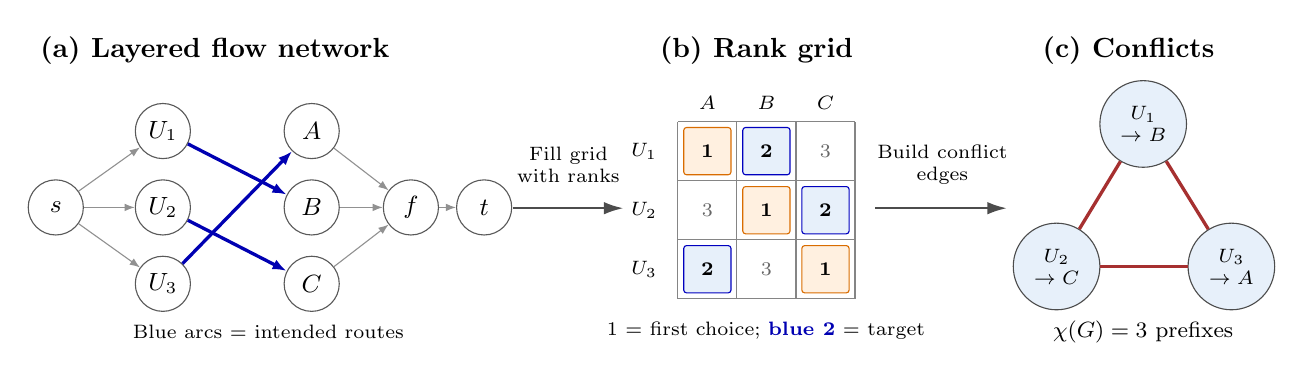
\begin{tikzpicture}[
  font=\small,
  flowNode/.style={circle,draw=black!65,fill=white,minimum size=7mm,inner sep=1pt},
  ordinaryFlow/.style={draw=black!43,thin,-{Latex[length=1.3mm]}},
  selectedFlow/.style={draw=blue!70!black,very thick,-{Latex[length=1.8mm]}},
  targetRank/.style={rectangle,rounded corners=1pt,draw=blue!75!black,fill=bluefill,
                     minimum width=6mm,minimum height=6mm,inner sep=0pt,font=\bfseries\scriptsize},
  firstRank/.style={rectangle,rounded corners=1pt,draw=orange!85!black,fill=orange!12,
                    minimum width=6mm,minimum height=6mm,inner sep=0pt,font=\bfseries\scriptsize},
  graphVertex/.style={circle,draw=black!70,fill=bluefill,minimum size=11mm,align=center,font=\scriptsize},
  conflict/.style={draw=redline,very thick},
  stageArrow/.style={-{Latex[length=2.5mm,width=1.6mm]},line width=.85pt,draw=black!70}
]
% Three panels, with the transformations explicitly named.
\node[anchor=west,font=\bfseries] at (-.10,3.80) {(a) Layered flow network};
\node[anchor=west,font=\bfseries] at (7.77,3.80) {(b) Rank grid};
\node[anchor=west,font=\bfseries] at (12.63,3.80) {(c) Conflicts};
% (a) Only the chosen U->ingress arcs are shown.
\node[flowNode] (s)  at (.22,1.81) {$s$};
\node[flowNode] (u1) at (1.58,2.78) {$U_1$};
\node[flowNode] (u2) at (1.58,1.81) {$U_2$};
\node[flowNode] (u3) at (1.58,.84) {$U_3$};
\node[flowNode] (a)  at (3.47,2.78) {$A$};
\node[flowNode] (b)  at (3.47,1.81) {$B$};
\node[flowNode] (c)  at (3.47,.84) {$C$};
\node[flowNode] (f)  at (4.73,1.81) {$f$};
\node[flowNode] (t)  at (5.66,1.81) {$t$};
\foreach \n in {u1,u2,u3} {\draw[ordinaryFlow] (s)--(\n);}
\foreach \n in {a,b,c} {\draw[ordinaryFlow] (\n)--(f);}
\draw[ordinaryFlow] (f)--(t);
\draw[selectedFlow] (u1)--(b);
\draw[selectedFlow] (u2)--(c);
\draw[selectedFlow] (u3)--(a);
\node[font=\scriptsize,align=center] at (2.92,.23) {Blue arcs = intended routes};
% (a) -> (b): two sources of information, not just a relabeling.
\draw[stageArrow] (6.03,1.80)--(7.43,1.80);
\node[font=\scriptsize,align=center] at (6.73,2.35)
  {Fill grid\\with ranks};
% (b) Ranks in every cell: smaller is preferred. Blue 2 = intended target.
\foreach \i in {0,...,3} {
  \draw[black!48] (8.12+.75*\i,.65)--(8.12+.75*\i,2.90);
  \draw[black!48] (8.12,.65+.75*\i)--(10.37,.65+.75*\i);
}
\foreach \lab/\i in {A/0,B/1,C/2}
  {\node[font=\scriptsize] at (8.495+.75*\i,3.14) {$\lab$};}
\foreach \lab/\i in {1/0,2/1,3/2}
  {\node[font=\scriptsize,anchor=east] at (7.98,2.525-.75*\i) {$U_{\lab}$};}
% U1: A > B > C; target B
\node[firstRank] at (8.495,2.525) {1};
\node[targetRank] at (9.245,2.525) {2};
\node[font=\scriptsize,text=black!60] at (9.995,2.525) {3};
% U2: B > C > A; target C
\node[font=\scriptsize,text=black!60] at (8.495,1.775) {3};
\node[firstRank] at (9.245,1.775) {1};
\node[targetRank] at (9.995,1.775) {2};
% U3: C > A > B; target A
\node[targetRank] at (8.495,1.025) {2};
\node[font=\scriptsize,text=black!60] at (9.245,1.025) {3};
\node[firstRank] at (9.995,1.025) {1};
\node[font=\scriptsize,align=center] at (9.24,.25)
  {1 = first choice; \textcolor{blue!70!black}{\textbf{blue 2}} = target};
% (b) -> (c): explain why each graph edge exists.
\draw[stageArrow] (10.63,1.80)--(12.30,1.80);
\node[font=\scriptsize,align=center] at (11.48,2.35)
  {Build conflict\\edges};
% (c) One vertex per intended assignment, red links are conflicts.
\node[graphVertex] (v1) at (14.03,2.87) {$U_1$\\$\to B$};
\node[graphVertex] (v2) at (12.93,1.06) {$U_2$\\$\to C$};
\node[graphVertex] (v3) at (15.15,1.06) {$U_3$\\$\to A$};
\draw[conflict] (v1)--(v2);
\draw[conflict] (v2)--(v3);
\draw[conflict] (v3)--(v1);
\node[font=\footnotesize,align=center] at (14.03,.23)
  {$\chi(G)=3$ prefixes};
\end{tikzpicture}%
}
\caption{How a full-control solution becomes a conflict graph.
(a) The chosen user--ingress flows are $U_1\to B$, $U_2\to C$, and $U_3\to A$.
(b) Each chosen arc identifies a \emph{target} (blue cell); the user's independent preference ordering supplies the ranks (1 = most preferred). All three targets have rank 2.
(c) Keep one vertex per target. An edge is added when one user's first choice is the ingress targeted by the other user. Every pair conflicts, so exact realization needs three prefixes.}
\label{fig:flow-to-conflict}
\end{figure}


\section{Exact realization is graph coloring}
\label{sec:graph}

\subsection{When do two intended assignments conflict?}

Consider two assignment components $v=(U,o)$ and $v'=(U',o')$ with $o\ne o'$. If they use the same prefix, both $o$ and $o'$ must announce it. They can share that prefix \emph{only if} $U$ does not prefer $o'$ over $o$ and $U'$ does not prefer $o$ over $o'$. Thus we create a conflict edge whenever
\begin{equation}\label{eq:edge}
v\sim v'
\quad\Longleftrightarrow\quad
o'\succ_U o\quad\text{or}\quad o\succ_{U'}o'.
\end{equation}
Assignments targeting the same ingress do not conflict. Let $G$ denote the resulting undirected \emph{assignment conflict graph}: its vertices are the positive components of $a^\star$, not the ingress options themselves.

\paragraph{Why the example requires three prefixes.}
In Figure~\ref{fig:flow-to-conflict}, each group is assigned its second choice:
$A\succ_{U_1} B$, $B\succ_{U_2} C$, and $C\succ_{U_3} A$.
Every pair of the three target assignments conflicts. For example, $(U_1,B)$ and $(U_3,A)$ cannot share a prefix: because $A$ must announce that prefix for $U_3$, $U_1$ would choose $A$ rather than $B$. Similarly, $(U_2,C)$ conflicts with $(U_1,B)$, and $(U_3,A)$ conflicts with $(U_2,C)$. This gives the triangle in panel (c).



\begin{lemma}[Exact prefix realization]\label{lem:color}
Assume strict, prefix-independent rankings and that a prefix announces exactly the distinct intended options of its assignment class. A partition of the assignment components preserves every intended route if and only if every class is an independent set of $G$. Consequently the minimum number of prefixes needed for exact realization is $\chi(G)$.
\end{lemma}
\begin{proof}
If a class has no conflict edge, then no component prefers another component's intended option over its own. Every component therefore chooses its target among all options announced for that class. Conversely, if a class contains both endpoints of a conflict edge, at least one endpoint prefers the other's intended option and is redirected. A partition into independent sets is exactly a proper vertex coloring, with each color representing one prefix.
\end{proof}

Announcing a class's prefix at options beyond its intended ones never helps. Under strict rankings, an extra option either ranks below the target of every component in the class, and then no component uses it, or it ranks above some component's target and takes that component's traffic.

The conflict graph characterizes whether a prefix allocation preserves the target routing decisions rather than their total cost. Two different routes may incur the same penalty, so a prefix allocation can change the target assignments without changing the objective value. Throughout, we use ``exact realization'' to mean preserving the target assignments themselves, not only their total cost. This matters beyond ties: moving traffic to an option with the same penalty can still overload that option or its facility, violating $\kappa_o$ or $\kappa_f$.

\subsection{The simpler, but coarser, ingress graph}

Let $A(v)$ denote the intended ingress of component $v$, and let
\[
\Sset=\{A(v):v\in V(G)\},\qquad M=|\Sset|.
\]
Coloring every component by its intended ingress is always valid; hence
\begin{equation}\label{eq:M}
\chi(G)\le M.
\end{equation}
One may also build a \emph{flattened ingress graph} $F$ whose vertices are the ingresses in $\Sset$: join $A$ and $B$ if some component intended for $A$ prefers $B$, or vice versa. Every coloring of $F$ induces a valid coloring of $G$: give each component the color of its intended ingress. Components with the same intended ingress never conflict, and a conflict between a component intended for $A$ and one intended for $B$ is exactly an edge $A$--$B$ of $F$, so no conflict edge of $G$ lies inside a color class. This gives
\begin{equation}\label{eq:flatten}
\chi(G)\le\chi(F)\le M.
\end{equation}
The reverse inequality need not hold, since coloring $F$ forces \emph{all} components assigned to the same ingress to share a color, whereas $G$ may place them on different prefixes and use fewer colors overall. We keep these two graphs distinct in the proofs below.

\begin{figure}[tbp]
\centering
\resizebox{\linewidth}{!}{%
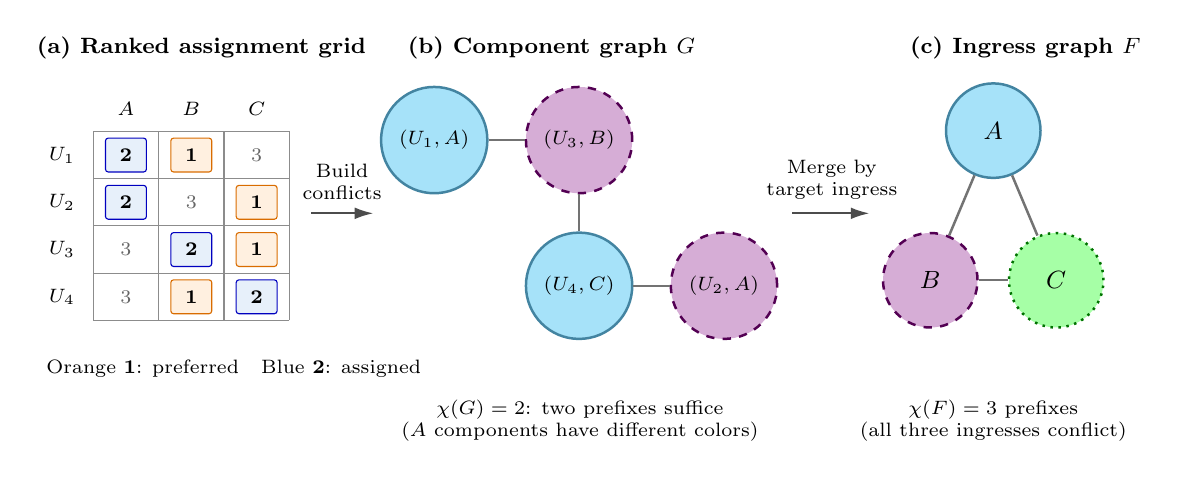
\begin{tikzpicture}[
  font=\small,
  targetRank/.style={rectangle,rounded corners=1pt,draw=blue!75!black,
    fill=bluefill,minimum width=5.2mm,minimum height=4.3mm,
    inner sep=0pt,font=\bfseries\scriptsize},
  firstRank/.style={rectangle,rounded corners=1pt,draw=orange!85!black,
    fill=orange!12,minimum width=5.2mm,minimum height=4.3mm,
    inner sep=0pt,font=\bfseries\scriptsize},
  graphVertex/.style={circle,draw=black!65,minimum size=13.5mm,
    inner sep=1pt,font=\scriptsize,align=center},
  ingressVertex/.style={circle,draw=black!65,minimum size=12mm,
    inner sep=1pt,font=\bfseries\small},
  prefixOne/.style={fill=cyan!35,draw=cyan!60!black,line width=.9pt},
  prefixTwo/.style={fill=violet!32,draw=violet!65!black,line width=.9pt,dashed},
  prefixThree/.style={fill=green!35,draw=green!45!black,line width=.9pt,dotted},
  conflictEdge/.style={draw=black!55,line width=.9pt},
  stageArrow/.style={-{Latex[length=2.4mm,width=1.5mm]},
    line width=.85pt,draw=black!70}
]
% Panel headings.
\node[anchor=west,font=\bfseries\footnotesize] at (.08,5.10) {(a) Ranked assignment grid};
\node[anchor=west,font=\bfseries\footnotesize] at (4.79,5.10) {(b) Component graph $G$};
\node[anchor=west,font=\bfseries\footnotesize] at (11.17,5.10) {(c) Ingress graph $F$};

% (a) Four assignments, all to second-choice ingresses:
% U1: B > A > C, U2: C > A > B,
% U3: C > B > A, U4: B > C > A.
% An orange 1 is a user's first choice; a blue 2 is its intended ingress.
\def\leftx{.92}
\def\bottomy{1.64}
\def\cw{.83}
\def\rh{.60}
\foreach \i in {0,...,3} {
  \draw[black!45] (\leftx+\cw*\i,\bottomy)--(\leftx+\cw*\i,\bottomy+4*\rh);
}
\foreach \j in {0,...,4} {
  \draw[black!45] (\leftx,\bottomy+\rh*\j)--(\leftx+3*\cw,\bottomy+\rh*\j);
}
\foreach \j/\colname in {1/A,2/B,3/C} {
  \pgfmathsetmacro{\xx}{\leftx+\cw*(\j-.5)}
  \node[font=\scriptsize] at (\xx,4.33) {$\colname$};
}
% row index / first-choice column / target column
\foreach \u/\first/\target/\r in {1/2/1/0,2/3/1/1,3/3/2/2,4/2/3/3} {
  \pgfmathsetmacro{\yy}{\bottomy+\rh*(3.5-\r)}
  \node[font=\scriptsize,anchor=east] at (.81,\yy) {$U_{\u}$};
  \pgfmathsetmacro{\xxfirst}{\leftx+\cw*(\first-.5)}
  \pgfmathsetmacro{\xxtarget}{\leftx+\cw*(\target-.5)}
  \node[firstRank] at (\xxfirst,\yy) {1};
  \node[targetRank] at (\xxtarget,\yy) {2};
  \pgfmathtruncatemacro{\third}{6-\first-\target}
  \pgfmathsetmacro{\xxthird}{\leftx+\cw*(\third-.5)}
  \node[font=\scriptsize,text=black!60] at (\xxthird,\yy) {3};
}
\node[font=\scriptsize,anchor=west] at (.20,1.03)
  {Orange \textbf{1}: preferred\quad Blue \textbf{2}: assigned};

% Ranked assignments -> component graph.
\draw[stageArrow] (3.69,3.00)--(4.48,3.00);
\node[font=\scriptsize,align=center] at (4.08,3.40) {Build\\conflicts};

% (b) Component graph is a path on four vertices:
% (U1,A)--(U3,B)--(U4,C)--(U2,A).
% Two prefixes suffice, and the two components targeting A have different colors.
\node[graphVertex,prefixOne] (v1) at (5.25,3.93) {$(U_1,A)$};
\node[graphVertex,prefixTwo] (v3) at (7.09,3.93) {$(U_3,B)$};
\node[graphVertex,prefixOne] (v4) at (7.09,2.08) {$(U_4,C)$};
\node[graphVertex,prefixTwo] (v2) at (8.93,2.08) {$(U_2,A)$};
\draw[conflictEdge] (v1)--(v3);
\draw[conflictEdge] (v3)--(v4);
\draw[conflictEdge] (v4)--(v2);
\node[font=\scriptsize,align=center] at (7.10,.37)
  {$\chi(G)=2$: two prefixes suffice\\($A$ components have different colors)};

% Component graph -> flattened ingress graph.
\draw[stageArrow] (9.80,3.00)--(10.78,3.00);
\node[font=\scriptsize,align=center] at (10.30,3.43)
  {Merge by\\target ingress};

% (c) The three ingress-level edges form K3, so three colors are needed.
\node[ingressVertex,prefixOne]   (a) at (12.35,4.05) {$A$};
\node[ingressVertex,prefixTwo]   (b) at (11.55,2.15) {$B$};
\node[ingressVertex,prefixThree] (c) at (13.15,2.15) {$C$};
\draw[conflictEdge] (a)--(b);
\draw[conflictEdge] (a)--(c);
\draw[conflictEdge] (b)--(c);
\node[font=\scriptsize,align=center] at (12.35,.37)
  {$\chi(F)=3$ prefixes\\(all three ingresses conflict)};
\end{tikzpicture}%
}
\caption{Flattening the conflict graph can increase the required number of prefixes.
(a) Every user is assigned to its second-choice ingress (blue~\textbf{2});
its first choice is shown in orange and its third choice in gray.
(b) The four assignment components form the path
$(U_1,A)$--$(U_3,B)$--$(U_4,C)$--$(U_2,A)$, which can be colored using two prefixes.
Vertex fill and outline style (solid, dashed, dotted) indicate prefix assignments. In particular, the two components assigned to $A$ use different prefixes.
(c) Merging all components with the same intended ingress produces the
flattened ingress graph $F$: the three pairwise conflicts $A$--$B$,
$B$--$C$, and $A$--$C$ form a triangle, requiring three colors.
Thus $\chi(G)=2<\chi(F)=3$.}
\label{fig:ingress-flattening}
\end{figure}

\section{Why assignment rank alone is not enough}
\label{sec:rank}

For an intended assignment $(U,A)$, let $r_U(A)$ be the rank of $A$ in $U$'s strict ordering (rank $1$ is best; the score $\pi_o(U)$ of Section~\ref{sec:model} runs the other way, with larger values more preferred, as in the main COMPASS paper), Only ingresses that are actually used can redirect a group, so we count rank among them. Assuming at least one positive assignment component (so $M\ge1$), define the \emph{active rank}
\[
k_U(A)=1+\bigl|\{B\in\Sset:B\succ_U A\}\bigr|\le r_U(A),
\qquad
K=\max_{(U,A)\in V(G)}k_U(A),
\]
where $\Sset$ is the set of ingresses used by the target (Section~\ref{sec:graph}). Thus $K-1$ is the largest number of used ingresses that any group ranks above its target. The full rank $r_U(A)$ also counts ingresses that no group is assigned to, and on measured deployments it can be far larger; Section~\ref{sec:agreement} uses it only for global agreement, where we write $\bar K=\max_{(U,A)\in V(G)}r_U(A)\ge K$.

If $K=2$, each user prefers at most one used ingress to its target. It is tempting to conclude that few prefixes should suffice. The triangle already demonstrates that three prefixes can be necessary for $K=2$. The next construction shows that there is \emph{no bound at all} that depends only on $K$.

\subsection{The shift-graph construction}

Take $n$ ingresses $A_1,\ldots,A_n$. For every pair $1\le i<j\le n$, create one user $U_{ij}$ assigned to $A_j$, with $A_i$ ranked first and $A_j$ second; all other ingresses rank below $A_j$. Represent its assignment vertex by $(i,j)$.

A vertex $(i,j)$ conflicts with $(h,i)$ whenever $h<i$: the user $U_{ij}$ prefers $A_i$, which is the intended ingress of $(h,i)$. Thus the conflict graph has exactly the edges
\begin{equation}\label{eq:shiftedges}
V(G_n)=\{(i,j):i<j\},\qquad
E(G_n)=\bigl\{\{(h,i),(i,j)\}:h<i<j\bigr\}.
\end{equation}
Figure~\ref{fig:shift} gives the small $n=5$ example. Unlike the three-user triangle, this graph is triangle-free; nevertheless, the highlighted odd cycle shows it cannot be colored with only two colors.

% Shift-graph figure (fig:shift). Requires tikz (arrows.meta), graphicx, float,
% and the colors bluefill and redline from the COMPASS preamble.
\begin{figure}[tbp]
\centering
\resizebox{\linewidth}{!}{%
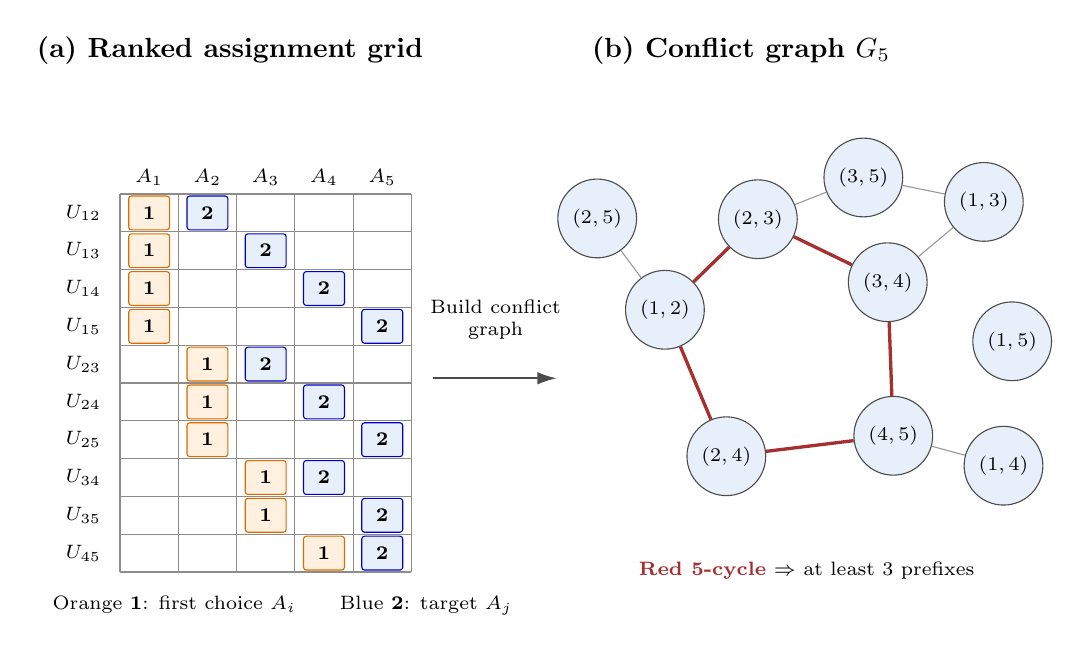
\begin{tikzpicture}[
  font=\small,
  targetRank/.style={rectangle,rounded corners=1pt,draw=blue!75!black,fill=bluefill,
                     minimum width=5.2mm,minimum height=4.3mm,inner sep=0pt,font=\bfseries\scriptsize},
  firstRank/.style={rectangle,rounded corners=1pt,draw=orange!85!black,fill=orange!12,
                    minimum width=5.2mm,minimum height=4.3mm,inner sep=0pt,font=\bfseries\scriptsize},
  graphVertex/.style={circle,draw=black!70,fill=bluefill,minimum size=10mm,inner sep=1pt,font=\scriptsize},
  otherEdge/.style={draw=black!40,thin},
  cycleEdge/.style={draw=redline,very thick},
  stageArrow/.style={-{Latex[length=2.5mm,width=1.6mm]},line width=.85pt,draw=black!70}
]
% Panel titles.
\node[anchor=west,font=\bfseries] at (.15,7.07) {(a) Ranked assignment grid};
\node[anchor=west,font=\bfseries] at (7.20,7.07) {(b) Conflict graph $G_5$};

% (a) Ten user groups: one group U_ij for every i<j.
% Orange 1 = U_ij prefers A_i most; blue 2 = U_ij is assigned to A_j.
\def\leftx{1.33}
\def\bottomy{.45}
\def\cw{.74}
\def\rh{.48}
\foreach \i in {0,...,5} {
  \draw[black!45] (\leftx+\cw*\i,\bottomy)--(\leftx+\cw*\i,\bottomy+10*\rh);
}
\foreach \j in {0,...,10} {
  \draw[black!45] (\leftx,\bottomy+\rh*\j)--(\leftx+5*\cw,\bottomy+\rh*\j);
}
\foreach \j in {1,...,5} {
  \pgfmathsetmacro{\xx}{\leftx+\cw*(\j-.5)}
  \node[font=\scriptsize] at (\xx,5.46) {$A_{\j}$};
}
\foreach \i/\j/\r in {1/2/0,1/3/1,1/4/2,1/5/3,2/3/4,
                          2/4/5,2/5/6,3/4/7,3/5/8,4/5/9} {
  \pgfmathsetmacro{\yy}{\bottomy+\rh*(9.5-\r)}
  \node[font=\scriptsize,anchor=east] at (1.21,\yy) {$U_{\i\j}$};
  \pgfmathsetmacro{\firstx}{\leftx+\cw*(\i-.5)}
  \pgfmathsetmacro{\targetx}{\leftx+\cw*(\j-.5)}
  \node[firstRank] at (\firstx,\yy) {1};
  \node[targetRank] at (\targetx,\yy) {2};
}
\node[font=\scriptsize,align=left,anchor=west] at (.35,.02)
  {Orange \textbf{1}: first choice $A_i$\qquad Blue \textbf{2}: target $A_j$};

% Grid -> graph transformation.
\draw[stageArrow] (5.30,2.91)--(6.88,2.91);
\node[font=\scriptsize,align=center] at (6.10,3.65) {Build conflict\\graph};

% (b) One vertex (i,j) for each blue target cell in the grid.
% Arrange the five vertices of the odd cycle around a clear pentagon.
\node[graphVertex] (n12) at (8.25,3.78) {$(1,2)$};
\node[graphVertex] (n23) at (9.43,4.93) {$(2,3)$};
\node[graphVertex] (n34) at (11.08,4.13) {$(3,4)$};
\node[graphVertex] (n45) at (11.15,2.18) {$(4,5)$};
\node[graphVertex] (n24) at (9.03,1.92) {$(2,4)$};
% Remaining vertices.
\node[graphVertex] (n25) at (7.39,4.94) {$(2,5)$};
\node[graphVertex] (n14) at (12.55,1.80) {$(1,4)$};
\node[graphVertex] (n13) at (12.30,5.15) {$(1,3)$};
\node[graphVertex] (n35) at (10.77,5.46) {$(3,5)$};
\node[graphVertex] (n15) at (12.66,3.38) {$(1,5)$};

% ALL five edges not on the highlighted odd cycle.
\foreach \p/\q in {n12/n25,n13/n34,n13/n35,n14/n45,n23/n35} {
  \draw[otherEdge] (\p)--(\q);
}
% Highlight the five-cycle, including the explicit closing edge n24--n12.
% (1,2)--(2,3)--(3,4)--(4,5)--(2,4)--(1,2)
\draw[cycleEdge] (n12)--(n23);
\draw[cycleEdge] (n23)--(n34);
\draw[cycleEdge] (n34)--(n45);
\draw[cycleEdge] (n45)--(n24);
\draw[cycleEdge] (n24)--(n12);

\node[font=\scriptsize,align=center] at (10.05,.47)
  {\textcolor{redline}{\textbf{Red 5-cycle}} $\Rightarrow$ at least 3 prefixes};
\end{tikzpicture}%
}
\caption{The shift-graph construction, using the same visual rules as Figure~\ref{fig:flow-to-conflict}.
For each $i<j$, user $U_{ij}$ ranks $A_i$ first and targets $A_j$ second; blank cells represent lower-ranked ingresses.
Each blue target cell becomes vertex $(i,j)$. Since $U_{ij}$ prefers $A_i$ to its assigned ingress, vertex $(i,j)$ conflicts with every vertex $(h,i)$ assigned to $A_i$.
The red five-cycle shows that $G_5$ cannot be $2$-colored even though every target has rank $2$; gray edges are the remaining conflicts. Three prefixes suffice, so $\chi(G_5)=3=\lceil\log_2 5\rceil$.}
\label{fig:shift}
\end{figure}

\begin{theorem}[Second choices can require arbitrarily many prefixes]\label{thm:shift}
For every $n\ge2$, there is an instance in which every user is assigned to its second-choice ingress, yet
\[
\chi(G_n)=\lceil\log_2 n\rceil.
\]
Therefore no upper bound on the number of prefixes required for exact realization can depend only on $K$.
\end{theorem}
\begin{proof}
Use the construction above, where every intended ingress has rank $2$. Suppose $G_n$ has a proper coloring with $c$ colors. For each ingress index $j$, collect the colors of the vertices assigned to $A_j$:
\[
C_j=\{\col(i,j):i<j\}\subseteq\{1,\ldots,c\},
\qquad C_1=\varnothing.
\]
The key observation is that these color sets must be \emph{different for every two ingress indices}. To see why, fix $i<j$. Vertex $(i,j)$ is adjacent to every vertex $(h,i)$, $h<i$, by Equation~\eqref{eq:shiftedges}. Its color is therefore absent from $C_i$. But $(i,j)$ is itself assigned to $A_j$, so its color belongs to $C_j$. Hence $C_i\ne C_j$.

In routing terms, $C_j$ is exactly the set of prefixes announced at $A_j$: under the announcement model of Lemma~\ref{lem:color}, a prefix is announced precisely at the intended ingresses of the components placed on it. The observation then says that to keep $U_{ij}$ on $A_j$, its prefix must be announced at $A_j$ but not at $A_i$, which $U_{ij}$ prefers. No two ingresses may therefore announce the same set of prefixes. Note the order of quantifiers: the instance is fixed, and the argument applies to \emph{every} proper coloring of $G_n$.

We have produced $n$ distinct subsets $C_1,\ldots,C_n$ of a palette of $c$ colors. Such a palette admits only $2^c$ distinct subsets. Consequently $n\le 2^c$, or $c\ge\lceil\log_2n\rceil$.

For the matching upper bound, color vertex $(i,j)$ by the lowest bit position at which $i-1$ has a $0$ and $j-1$ has a $1$; such a position exists because $i<j$. If $(h,i)$ and $(i,j)$ are adjacent, then $i-1$ has a $1$ at the color of $(h,i)$ and a $0$ at the color of $(i,j)$, so the two colors differ. Every color is a bit position of a number below $n$, so $\lceil\log_2 n\rceil$ colors suffice. ($G_n$ is the shift graph of Erd\H{o}s and Hajnal.) Since $n$ can grow without changing $K=2$, no function of $K$ alone bounds $\chi(G_n)$.
\end{proof}

The problem is \emph{collective compatibility}, not the number of better choices available to any single user. Even with one better alternative per user, those alternatives can interact across many assignments and force increasingly many colors.

\section{What preference agreement can guarantee}
\label{sec:agreement}

The impossibility theorem says that $K$ alone is insufficient. It does not say that every realistic preference profile needs many prefixes. We now identify two distinct properties that give useful upper bounds: \emph{global agreement} about which ingresses appear among users' top choices, and \emph{local agreement} about which alternatives are preferred by users assigned to the same ingress.

\subsection{Global agreement: how many different ingresses can be targets?}

Recall that $\Sset$ is the set of ingresses used by the target assignment and $M=|\Sset|$. By Equation~\eqref{eq:M}, $M$ prefixes always suffice: assign one prefix to all components targeting each distinct ingress.

\begin{proposition}[Identical rankings]\label{prop:identical}
If all users share the same strict ranking and every target has active rank at most $K$, then
\[
\chi(G)=M\le K.
\]
\end{proposition}
\begin{proof}
In the common ranking, the lowest-ranked intended ingress has the other $M-1$ intended ingresses above it, so its active rank is $M$ and $M\le K$. Now take one assignment vertex for each distinct intended ingress. For any two different ingresses, a user assigned to the lower-ranked one prefers the higher-ranked one. The chosen vertices therefore form an $M$-clique, giving $\chi(G)\ge M$. Together with $\chi(G)\le M$, this proves equality.
\end{proof}

Identical rankings are stronger than necessary to obtain an upper bound in terms of rank. The remaining global results count rank among \emph{all} ingresses, so they use the full rank $\bar K$ of Section~\ref{sec:rank}. If every user's top-$\bar K$ \emph{set} is the same set $T$ of size $\bar K$, users may disagree on its internal order, but every target still belongs to $T$. Thus $M\le \bar K$ and $\chi(G)\le \bar K$. Equality need not hold because disagreements about the order can eliminate conflicts.

More generally, partition the user groups into \emph{preference types}: groups of the same type share the same ranking, or at least the same set of top $\bar K$ ingresses. Let $\tau$ be the number of types and $T_t$ the top-$\bar K$ set of type $t$, and define the \emph{top-$\bar K$ diversity}
\[
M_{\bar K}=\left|\bigcup_{t=1}^{\tau}T_t\right|.
\]
Every intended ingress occurs in some user's top-$\bar K$ set; hence
\begin{equation}\label{eq:global}
\boxed{\chi(G)\le M\le M_{\bar K}\le \tau \bar K.}
\end{equation}
This single observation includes the common-set case ($M_{\bar K}=\bar K$) and the case of two preference types. For two types with $|T_1\cap T_2|=m$,
\begin{equation}\label{eq:two}
\chi(G)\le |T_1\cup T_2|=2\bar K-m.
\end{equation}
The more their sets overlap, the fewer distinct target ingresses can appear. These are upper bounds, not exact prefix counts: the target ingresses may be numerous without all conflicting.

\subsection{Local agreement: how many better alternatives compete with an ingress?}

The bound $\chi(G)\le M$ can be loose if COMPASS uses many ingresses whose assignments can nevertheless share prefixes. We need a measure of how their preferences interact.

For each assigned ingress $A\in\Sset$, define its set of \emph{aggregated better assigned alternatives}
\begin{equation}\label{eq:H}
H(A)=\bigcup_{v=(U,A)}\bigl\{B\in\Sset:B\succ_U A\bigr\},
\qquad
R=\max_{A\in\Sset}|H(A)|.
\end{equation}
Only alternatives that are themselves assigned somewhere in the target matter: if no component needs ingress $B$ to be announced, the assignment can omit $B$ from every prefix.

The distinction between $K$ and $R$ is crucial. When every target has active rank at most $K$, an individual user prefers at most $K-1$ used alternatives. But \emph{different users assigned to the same ingress} may prefer different alternatives. Their union $H(A)$ may therefore be much larger than $K-1$.

Figure~\ref{fig:local} shows the aggregation required by the proof. It is deliberately drawn on \emph{ingresses} rather than on individual assignment components: the next theorem colors the flattened graph $F$.

\begin{figure}[tbp]
\centering
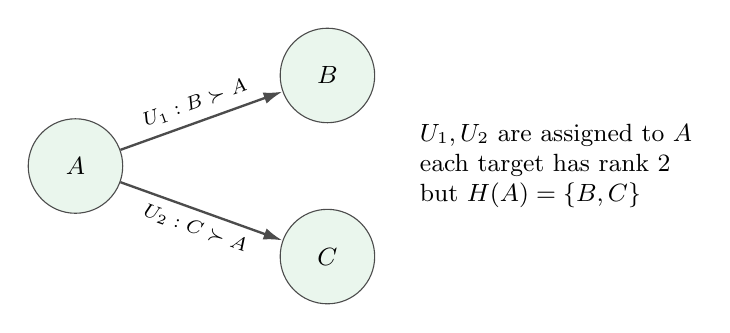
\begin{tikzpicture}[
  ingress/.style={circle,draw=black!70,fill=greenfill,minimum size=12mm,font=\small},
  arrow/.style={-{Latex[length=2.4mm,width=1.5mm]},line width=.85pt,draw=black!70}]
\node[ingress] (A) at (0,0) {$A$};
\node[ingress] (B) at (3.2,1.15) {$B$};
\node[ingress] (C) at (3.2,-1.15) {$C$};
\draw[arrow] (A) -- node[above,sloped,font=\scriptsize] {$U_1:B\succ A$} (B);
\draw[arrow] (A) -- node[below,sloped,font=\scriptsize] {$U_2:C\succ A$} (C);
\node[anchor=west,align=left,font=\small] at (4.25,0) {$U_1,U_2$ are assigned to $A$\\each target has rank $2$\\but $H(A)=\{B,C\}$};
\end{tikzpicture}
\caption{Local preference diversity aggregates \emph{across} users with the same target. Each user assigned to $A$ has only one better alternative ($K=2$), but the union of their better assigned alternatives has size two. Here $B$ and $C$ are assumed to be targets of other users, so $B,C\in\Sset$. The theorem bounds the outdegree of this directed ingress graph, not the outdegree of a user-assignment vertex.}
\label{fig:local}
\end{figure}

\begin{theorem}[Bounded local preference diversity]\label{thm:local}
Recall that $M=|\Sset|$ is the number of ingresses used by the target assignment. If $|H(A)|\le R$ for every assigned ingress $A$, then
\[
\boxed{\chi(G)\le\min\{M,2R+1\}.}
\]
\end{theorem}
\begin{proof}
The hypothesis bounds how many ingresses the users of each ingress would defect to, not how many ingresses conflict with it: in $F$ an ingress can have arbitrarily high degree. We therefore keep track of direction. Construct the directed graph $\vec F$ on the assigned ingresses $\Sset$, with an arc $A\to B$ whenever $B\in H(A)$, i.e., whenever some component intended for $A$ prefers $B$. Every vertex has outdegree at most $R$. Ignoring the directions gives exactly the flattened conflict graph $F$ of Section~\ref{sec:graph}.

Consider any nonempty subset $X\subseteq\Sset$. Its induced directed subgraph contains at most $R|X|$ arcs: each vertex in $X$ has at most $R$ outgoing arcs, including those leaving $X$. Every undirected edge of $F[X]$ is represented by at least one arc, so
\[
|E(F[X])|\le R|X|.
\]
The average degree in $F[X]$ is thus at most $2R$. Every nonempty induced subgraph of $F$ therefore contains a vertex of degree at most $2R$. Removing such a vertex repeatedly, and coloring in reverse removal order, uses at most $2R+1$ colors. Hence $\chi(F)\le 2R+1$. Finally, Equation~\eqref{eq:flatten} gives $\chi(G)\le\chi(F)\le2R+1$, and Equation~\eqref{eq:M} also gives $\chi(G)\le M$.
\end{proof}

This is the correct form of the bounded-outdegree argument: the relevant outdegree is aggregated at the \emph{ingress} level. A user-level outdegree of at most $K-1$ does not imply the ingress-level bound $R\le K-1$; the shift-graph construction demonstrates why. There, every target has rank $2$, yet $H(A_j)=\{A_1,\ldots,A_{j-1}\}$, so $R=n-1$ and Theorem~\ref{thm:local} gives only $\chi(G_n)\le n$. This is consistent with Theorem~\ref{thm:shift}: the bound is valid but uninformative when users assigned to the same ingress prefer many different alternatives. The bound $2R+1$ is tight for $\chi(F)$: with $R=1$ the ingress graph can be an odd cycle, and in general a regular tournament on $2R+1$ ingresses has every outdegree equal to $R$ and a complete underlying graph, so $\chi(F)=2R+1$. The true $\chi(G)$ can still be smaller.

The theorem bounds $\chi(F)$, i.e., the number of prefixes needed when all components assigned to an ingress share one prefix. Since $\chi(F)$ can exceed $\chi(G)$ (Figure~\ref{fig:ingress-flattening}), $\min\{M,2R+1\}$ is a sufficient prefix budget, not the exact number of prefixes required.

\subsection{When does the $2K-1$ bound hold?}

\begin{corollary}[Local agreement]\label{cor:agreement}
Suppose every target has active rank at most $K$ and all users assigned to the same ingress $A$ agree on the set of ingresses ranked above $A$. Then
\[
\chi(G)\le\min\{M,2K-1\}.
\]
\end{corollary}
\begin{proof}
For each $A$, the common better-choice set contains at most $K-1$ used ingresses, so $|H(A)|\le K-1$. Apply Theorem~\ref{thm:local}.
\end{proof}

This does \emph{not} require a global ranking shared by all users. Users assigned to different ingresses may disagree completely; what matters is that users with a common intended ingress do not introduce new competing alternatives into the union $H(A)$. This is precisely the hypothesis that the shift construction violates: there, each user assigned to $A_j$ prefers a different ingress.

We can weaken exact agreement. Choose one reference user $U_A$ for each assigned ingress $A$ and set
\[
H_0(A)=\{B\in\Sset:B\succ_{U_A}A\}.
\]
If every target has active rank at most $K$ and, for every $A$,
\[
|H(A)\setminus H_0(A)|\le\Delta,
\]
then $|H(A)|\le K-1+\Delta$. Hence
\begin{equation}\label{eq:delta}
\boxed{\chi(G)\le\min\{M,2K+2\Delta-1\}.}
\end{equation}
The parameter $\Delta$ counts \emph{distinct additional ingress labels}, not the number of users who disagree. It can remain small even when many users have different complete rankings.

Alternatively, suppose at most $\tau_{\rm loc}$ distinct preference types occur among users assigned to any single ingress. Each type contributes at most $K-1$ better alternatives, so $R\le \tau_{\rm loc}(K-1)$ and
\begin{equation}\label{eq:types}
\boxed{\chi(G)\le\min\{M,2\tau_{\rm loc}(K-1)+1\}.}
\end{equation}
Unlike the global bound $\tau \bar K$, this guarantee depends on how preferences vary \emph{within each assigned ingress}, not on the number of preference types in the population as a whole.

\subsection{Setting outlier ingresses aside}

The parameter $R$ is a maximum over all assigned ingresses. A single ingress whose users have many different better alternatives, such as a catch-all site that receives traffic from many regions, can therefore make Theorem~\ref{thm:local} uninformative even when every other ingress has few competitors. Giving such ingresses prefixes of their own removes them from the maximum.

\begin{corollary}[Setting outlier ingresses aside]\label{cor:outliers}
For any $S\subsetneq\Sset$, let
\[
R_S=\max_{A\in\Sset\setminus S}|H(A)\setminus S|.
\]
Then
\[
\chi(G)\le\chi(F)\le|S|+2R_S+1,
\qquad\text{hence}\qquad
\boxed{\chi(G)\le\min\Bigl\{M,\ \min_{S\subsetneq\Sset}\bigl(|S|+2R_S+1\bigr)\Bigr\}.}
\]
\end{corollary}
\begin{proof}
Give each ingress in $S$ a color of its own, used by no other ingress; then no edge of $F$ incident to $S$ joins two vertices of the same color. The induced subgraph $F-S$ is the flattened graph of the remaining ingresses, and in the directed graph $\vec F-S$ each vertex $A$ has outdegree $|H(A)\setminus S|\le R_S$. The argument of Theorem~\ref{thm:local} applied to $F-S$ colors it with at most $2R_S+1$ further colors, so $\chi(F)\le|S|+2R_S+1$. Equation~\eqref{eq:flatten} gives $\chi(G)\le\chi(F)$. Taking $S=\varnothing$ recovers Theorem~\ref{thm:local}.
\end{proof}

For example, if one ingress $X$ has $|H(X)|=50$ while every other ingress has $|H(A)|\le 2$, Theorem~\ref{thm:local} gives $101$ prefixes, whereas setting $X$ aside gives $1+2\cdot2+1=6$. Setting an ingress aside pays off when it is an outlier in \emph{outdegree}, i.e., when its own users disagree. A popular ingress that appears in many sets $H(A)$ lowers $R$ by at most one when removed, so setting it aside saves at most one prefix.

\subsection{Summary of the structural results}

The results describe different forms of preference agreement:
\begin{center}
\small
\begin{tabular}{@{}p{0.40\linewidth}p{0.45\linewidth}@{}}
\toprule
\textbf{Assumption} & \textbf{Exact-prefix guarantee}\\
\midrule
Identical strict rankings & $\chi(G)=M\le K$\\
Common top-$\bar K$ set (full rank) & $\chi(G)\le M\le \bar K$\\
Top-$\bar K$ diversity $M_{\bar K}$ & $\chi(G)\le M\le M_{\bar K}$\\
Local better-choice diversity $R$ & $\chi(G)\le\min\{M,2R+1\}$\\
Local agreement among users assigned to each ingress & $\chi(G)\le\min\{M,2K-1\}$\\
Few outlier ingresses $S$ set aside & $\chi(G)\le\min\{M,|S|+2R_S+1\}$\\
Common weak order with ties of size at most $w$ & $\chi(G)\le\min\{M,2K+2w-3\}$\\
Arbitrary rankings & No bound depending only on $K$\\
Arbitrary rankings, targets of active rank at most $K$ & $\chi(G)\le L_{K-1}(M)=O(K^2\log M)$\\
Any instance & $\lceil\log_2\chi(F)\rceil\le\chi(G)\le\chi(F)$\\
\bottomrule
\end{tabular}
\end{center}
In particular, global agreement keeps the \emph{number of distinct target ingresses} small. Local agreement permits many target ingresses but keeps the \emph{conflict structure} sparse enough to color with fewer prefixes. Neither parameter necessarily equals the true chromatic number.

A common partial order does not, by itself, rescue a rank-only guarantee. If it leaves all ingresses used in the shift construction incomparable, the users' strict rankings can extend that partial order while still generating $G_n$ with unbounded chromatic number. A useful hypothesis must restrict the comparisons that actually induce conflict edges. A common weak order does so when its ties are small: suppose every user's ranking extends a ranking of the ingresses into tied buckets, each of at most $w$ ingresses. An ingress $B$ in a strictly higher bucket than $A$ is ranked above $A$ by every user, so a user assigned to $A$ at active rank at most $K$ sees at most $K-1$ of them; the remaining members of $H(A)$ share $A$'s bucket. Hence $|H(A)|\le K+w-2$, and Theorem~\ref{thm:local} gives $\chi(G)\le\min\{M,2K+2w-3\}$. With $w=1$ the order is total and this recovers the $2K-1$ bound.

\section{How tight are these bounds?}
\label{sec:tightness}

The previous sections give upper bounds that rest on agreement, and Theorem~\ref{thm:shift} shows that rank alone cannot bound the number of prefixes independently of the instance. Two further results complete the picture. The ingress-level plan of Equation~\eqref{eq:flatten} is never more than exponentially worse than the best plan, and rank together with the number of used ingresses always gives a logarithmic bound.

\subsection{Flattening costs at most an exponential}

\begin{proposition}[Flattening sandwich]\label{prop:sandwich}
For every instance,
\[
\lceil\log_2\chi(F)\rceil\;\le\;\chi(G)\;\le\;\chi(F).
\]
\end{proposition}
\begin{proof}
The upper bound is Equation~\eqref{eq:flatten}. For the lower bound, fix a proper coloring of $G$ with $c=\chi(G)$ colors, and give each used ingress $A$ the set $C_A$ of colors used by components intended for $A$. Let $A$ and $B$ be adjacent in $F$; say some component $(U,B)$ has $A\succ_U B$. Its color belongs to $C_B$. It cannot belong to $C_A$, because a component intended for $A$ with that color would conflict with $(U,B)$. Hence $C_A\ne C_B$, so $A\mapsto C_A$ is a proper coloring of $F$ with at most $2^c$ distinct sets, and $\chi(F)\le 2^{\chi(G)}$.
\end{proof}

In routing terms, $C_A$ is the set of prefixes announced at $A$: any two ingresses joined in $F$ must announce different sets of prefixes. The proof of Theorem~\ref{thm:shift} is this argument applied to the shift instance, where $F$ is complete on the $n-1$ used ingresses. Both inequalities can be tight: identical rankings give $\chi(G)=\chi(F)=M$ (Proposition~\ref{prop:identical}), and the shift instance has $\chi(F)=n-1$ but $\chi(G_n)=\lceil\log_2 n\rceil$, so the lower bound is attained up to rounding.

\subsection{What rank does guarantee}

For $d\ge0$, call a list of sets \emph{$d$-cover-free} if no member is contained in the union of $d$ other members, and let $L_d(M)$ be the smallest $L$ for which $\{1,\dots,L\}$ has a $d$-cover-free list of $M$ subsets. Since the $M$ singletons form such a list, $L_d(M)\le M$.

\begin{theorem}[Rank gives a logarithmic bound]\label{thm:coverfree}
If every target has active rank at most $K$, then
\[
\chi(G)\le L_{K-1}(M).
\]
For $K=2$ this is $\chi(G)\le\min\bigl\{L:\binom{L}{\lfloor L/2\rfloor}\ge M\bigr\}=\log_2M+O(\log\log M)$, and in general $\chi(G)=O(K^2\log M)$.
\end{theorem}
\begin{proof}
Let $L=L_{K-1}(M)$ and give the used ingresses codes $c(A)\subseteq\{1,\dots,L\}$ forming a $(K-1)$-cover-free list. A component $(U,A)$ ranks at most $K-1$ used ingresses above $A$; call them $\mathcal B$. Because no code is covered by $K-1$ others, $c(A)\setminus\bigcup_{B\in\mathcal B}c(B)$ is nonempty: place $(U,A)$ on any prefix $p$ in it. Every component on prefix $p$ is intended for an ingress whose code contains $p$. If two components $(U,A)$ and $(U',B)$ on prefix $p$ conflicted, say with $B\succ_U A$, then $p\in c(B)$, contradicting the choice of $p$ for $(U,A)$. So the placement is a proper coloring of $G$ with $L$ colors.

For $K=2$, a $1$-cover-free list is an antichain of distinct sets, and by Sperner's theorem the largest antichain of subsets of $\{1,\dots,L\}$ has $\binom{L}{\lfloor L/2\rfloor}$ members. For general $d$, known constructions of $d$-cover-free families (Erd\H{o}s, Frankl and F\"uredi) give $L_d(M)=O(d^2\log M)$.
\end{proof}

In routing terms, $c(A)$ is the set of prefixes ingress $A$ may announce. A group is placed on a prefix that its target announces and that none of the ingresses it prefers announces, so the code length, not the number of ingresses, is what limits the prefix count. Unlike Theorem~\ref{thm:local}, this bound colors $G$ directly: components intended for the same ingress may use different prefixes. Together with Theorem~\ref{thm:shift}, it shows that for second-choice assignments the number of prefixes grows logarithmically in the number of ingresses: some instances need $\lceil\log_2 n\rceil$, and none needs more than about $\log_2 M$.

\section{What if the prefix budget is too small?}
\label{sec:budget}

When $B_{\rm prefix}<\chi(G)$, no partition can preserve every target route. The correct objective is then the cost of the \emph{actual winners}, not simply how many conflict edges lie inside each prefix class.

\subsection{Why pairwise edge penalties can mislead}

Suppose component $1$ targets $o_1$ but ranks $o_3\succ o_2\succ o_1$. Relative to the intended route, moving this component to $o_2$ costs $4$ and moving it to $o_3$ costs $6$. Another component, component $3$, targets $o_3$ but prefers $o_4$, at additional cost $5$. Assume the other relevant preference comparisons are nonconflicting and all intended costs are zero. The conflict edges have proxy weights $(1,2):4$, $(1,3):6$, and $(3,4):5$.

With two prefixes, consider
\begin{center}
\small
\begin{tabular}{@{}lccc@{}}
\toprule
Partition & Prefix classes & Sum of internal edge penalties & Actual cost\\
\midrule
(i) & $\{1,2,3\},\ \{4\}$ & $4+6=10$ & $6$\\
(ii) & $\{1,2\},\ \{3,4\}$ & $4+5=9$ & $4+5=9$\\
\bottomrule
\end{tabular}
\end{center}
The edge proxy chooses partition (ii), but the actual cost favors (i). In (i), component $1$ sees both $o_2$ and $o_3$ and chooses \emph{only} $o_3$. Its two incident edges describe alternative redirections, not two costs that can be added. The class's entire announcement set determines its winner.

\subsection{Exact fixed-target formulation}

Let $V$ be the atomic assignment components. For any nonempty class $S\subseteq V$, define
\[
\mathcal A(S)=\{o_v:v\in S\},\qquad
h_v(S)=\arg\max_{o\in\mathcal A(S)}\pi_o(U_v),
\]
where $\arg\max$ selects the most-preferred option in the announced set. Define its realized routing cost, regret relative to the target, and induced option/facility loads:
\begin{align}
g(S)&=\sum_{v\in S}w_v\phi(h_v(S),U_v),\label{eq:g}\\
\rho(S)&=\sum_{v\in S}w_v\bigl[\phi(h_v(S),U_v)-\phi(o_v,U_v)\bigr],\label{eq:rho}\\
\ell_o(S)&=\sum_{v\in S:\,h_v(S)=o}w_v,\label{eq:ell}\\
\ell_f(S)&=\sum_{o:f(o)=f}\ell_o(S).\label{eq:ellF}
\end{align}
(The regret $\rho(S)$ can be negative if an induced winner is cheaper than the full-control target for that component; the fixed target's total cost is constant in either case.)

Let $\mathcal C\subseteq2^V\setminus\{\varnothing\}$ be candidate prefix classes, and let $\theta_S\in\{0,1\}$ indicate whether class $S$ receives a prefix. The fixed-target realization problem is
\begin{equation}\label{eq:partition}
\begin{aligned}
\min_{\theta}\quad&\sum_{S\in\mathcal C}\rho(S)\theta_S\\
\text{s.t.}\quad&\sum_{S\ni v}\theta_S=1 &&\forall v\in V,\\
&\sum_{S\in\mathcal C}\theta_S\le B_{\rm prefix},\\
&\sum_{S\in\mathcal C}\ell_o(S)\theta_S\le\kappa_o &&\forall o\in D,\\
&\sum_{S\in\mathcal C}\ell_f(S)\theta_S\le\kappa_f &&\forall f,\\
&\theta_S\in\{0,1\} &&\forall S\in\mathcal C.
\end{aligned}
\end{equation}
The first two constraints partition all components into at most $B_{\rm prefix}$ prefix classes. The remaining constraints check capacities \emph{after} preference-induced redirection. Choosing all nonempty subsets makes this an exact, but exponential-size, set-partitioning formulation for the fixed target and the class-announcement policy. If arbitrary prefix classes are generated selectively, optimality holds only over the generated family.

\subsection{Practical approximation}

A scalable implementation can start by assigning vertices to at most $B_{\rm prefix}$ colors using conflict weights as an inexpensive heuristic. But after assigning the colors, it must reconstruct each color's set of announced options and recompute: (i) every component's actual winner, (ii) option and facility loads, and (iii) the true realized objective. Candidate moves include recoloring one component, swapping two colors, or moving all components targeting one ingress. A move should be accepted only if it preserves capacity feasibility and improves the \emph{actual} objective. If the goal is exact coloring and the prefix budget is not binding, DSATUR is a useful baseline.

The two-stage decomposition is not globally optimal for a fixed prefix budget. A deployment with a slightly worse full-control assignment may be much easier to realize and have a better final outcome. One extension is to incorporate a prefix-realization penalty into the infrastructure search; another is to jointly optimize deployment and prefix classes.

\section{Implications for COMPASS}

The mathematical results suggest concrete diagnostics for an empirical evaluation. For every full-control target, COMPASS can measure the maximum active rank $K$, the number $M$ of distinct targeted ingresses, the top-$\bar K$ diversity $M_{\bar K}$, the aggregated local diversity $R$, and the observed number of colors needed for exact realization. These measurements distinguish two explanations for small prefix budgets: either the assignment uses few ingresses, or it uses many ingresses whose conflicts permit substantial color reuse.

Preference rankings may change faster than physical deployment. COMPASS can first attempt to recolor a fixed deployment when rankings change, and trigger deployment optimization only when the resulting routes are too costly or violate capacity.

The main practical quantity is the \emph{realization gap}: how much the best available prefix scheme differs from the full-control target under the same infrastructure and capacities. Prefix realization is best understood as constrained menu design: the planner controls which options are visible together; each user chooses its preferred visible option. Rank by itself does not predict how many such menus are necessary. What matters is how the intended ingresses and the preferences for competing ingresses interact across the entire assignment.

\end{document}




